\documentclass{scrartcl}
\usepackage{tikz}
\usetikzlibrary{arrows, automata}
\usepackage{comment}
\usepackage{amsmath}

\begin{document}

Example 1:
 This is a \TeX file.

 \[
  (f\ast g) = \int_{-\infty}^{\infty} f{\tau} g(t-\tau) \, d\tau
 \]

Example 2:
\textit{As NFA defined on Page 54 of ITC}\\
textbook.\\

% begin math model
$
Q = \{q_1, q_2, q_3, q_4\} \\
\sum = \{0, 1\}\\
F = \{q_4\}\\
q_0 = q_1 \\
\delta = \{
            ((q_1, 0), \{q_1\}), ((q_1, 1), \{q_1, q_2\}), ((q_1, \epsilon), \phi), \\
            ((q_2, 0), \{q_3\}), ((q_2, 1),\phi), ((q_2, \epsilon), \{q_3\}), \\
            ((q_3, 0), \phi), ((q_3, 1), \{q_4\}), ((q_3, \epsilon), \phi), \\
            ((q_4, 0), \{q_4\}), ((q_4, 1), \{q_4\}), ((q_4, \epsilon), \phi)
\} \\
$
%end math model

Transition Function in Table form: \\
\begin{center}
  \begin{tabular}{||c c c c||}
    \hline
    \space  &0      &1              &$\epsilon$    \\[0.5ex]
    \hline
    $q_1$          & \{$q_1$\}      & \{$q_1$, $q_2$\}    &$\phi$        \\
    \hline
    $q_2$          & \{$q_3$\}      & $\phi$              & \{$q_3$\}    \\
    \hline
    $q_3$          & $\phi$         & \{$q_4$\}           & $\phi$       \\
    \hline
    $q_4$          & \{$q_4$\}      & \{$q_4$\}           & $\phi$       \\
    \hline
  \end{tabular}
\end{center}

NFA in pictorial form: \\

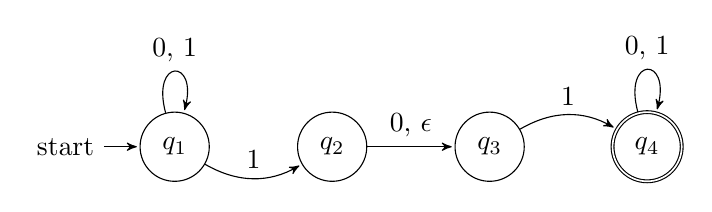
\begin{tikzpicture}[>=stealth',shorten >=1pt, auto, node distance=2cm]
  \node[initial, state]       (q1)                  {$q_1$};
  \node[state]                (q2)[right of=q1]     {$q_2$};
  \node[state]                (q3)[right of=q2]     {$q_3$};
  \node[state, accepting]     (q4)[right of=q3]     {$q_4$};

  \path[->](q1) edge [loop above]    node {0, 1}(q1)
                edge [bend right]    node {1} (q2)
          (q2)  edge                 node {0, $\epsilon$} (q3)
          (q3)  edge [bend left]     node {1} (q4) 
          (q4)  edge [loop above]    node {0, 1} (q4);
\end{tikzpicture}

Example 3:
 \textbf{\textit{DFA, state diagram of machine M}}
\begin{center}
  \begin{tikzpicture}[>=stealth',shorten >=2pt, auto, node distance=5cm]
    %define states in the machine
    \node[initial, state, accepting] (q3) {$q_3$};
    \node[state]  (q2) [above of= q3] {$q_2$};
    \node[state]  (q1) [right of= q2] {$q_1$};
    \node[state]  (q4) [below of=q3] {$q_4$};
    \node[state]  (q5) [right of=q4]  {$q_5$};

    %define the links
    \path[->] (q1) edge[loop above] node{u}  (q1)
                   edge             node{d}  (q2)
              (q2) edge[bend left]  node{u}  (q1)
                   edge             node{d}  (q3)
              (q3) edge[bend left]  node{u}  (q2)
                   edge             node{d}  (q4)
              (q4) edge[bend left]  node{u}  (q3)
                   edge             node{d}  (q5)
              (q5) edge[bend left]  node{u}  (q4)
                   edge[loop above] node{d}  (q5);
  \end{tikzpicture}
\end{center}

Example 4: 
\textbf{textit{Machine DFA has 02 languages and it combine:}}\\
\{w$|$ w has at least three a's\}\\
\begin{center}
  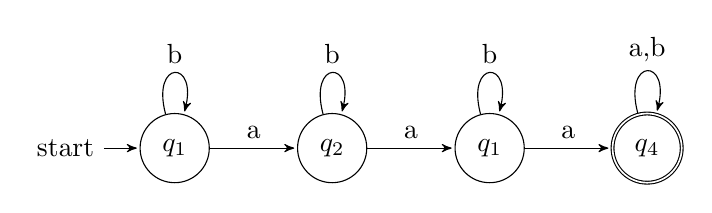
\begin{tikzpicture}[>=stealth',shorten >=1pt,auto, node distance=2cm]
    
    %define the state in the machine
    \node[initial, state] (q1) {$q_1$};
    \node[state]           (q2) [right of=q1] {$q_2$};
    \node[state]           (q3) [right of=q2] {$q_1$};
    \node[state, accepting] (q4) [right of=q3] {$q_4$};

    % define the links
    \path[->](q1)edge[loop above] node {b} (q1)   edge node{a} (q2)
    (q2) edge [loop above] node {b} (q2)
         edge node {a}(q3)
    (q3) edge [loop above] node {b} (q3)
         edge node{a} (q4)
    (q4) edge [loop above] node{a,b} (q4);
  \end{tikzpicture}
\end{center}

\{w$|$ has at least three b's\}\\
\begin{center}
  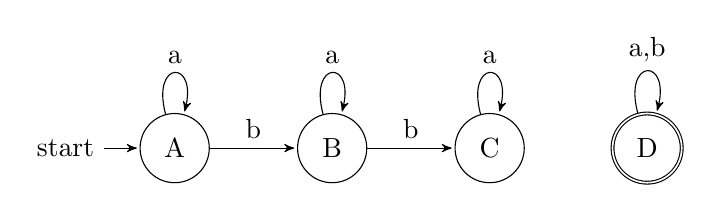
\begin{tikzpicture}[>=stealth', shorten >=1pt, auto, node distance=2cm]

    %define the states in the machine
    \node[initial, state] (q1)  {A};
    \node[state] (q2) [right of=q1] {B};
    \node[state] (q3) [right of=q2] {C};
    \node[state, accepting] (q4) [right of=q3] {D};

    %define the link
    \path[->](q1) edge [loop above] node {a} (q1)
    edge   node {b} (q2)
    (q2) edge [loop above] node {a} (q2)
    edge    node {b} (q3)
    (q3) edge [loop above] node {a} (q4)
    (q4) edge [loop above] node {a,b} (q4); 
  \end{tikzpicture}
\end{center}

Combining them using the intersection construction for DFA machine:\\
\begin{center}
  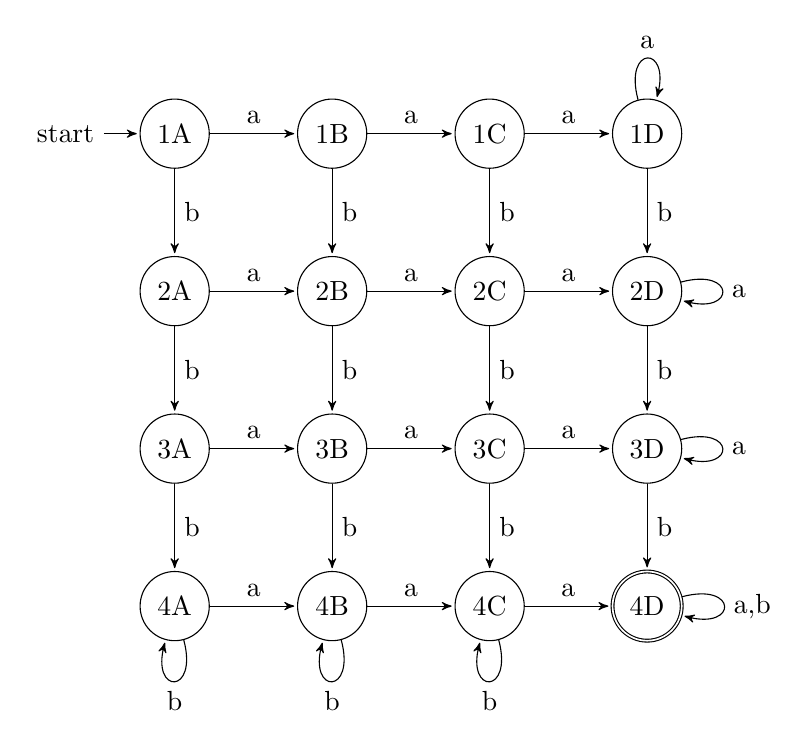
\begin{tikzpicture}[>=stealth', shorten >=1pt, auto, node distance=2cm]
    %define the states in the machine
    \node[initial, state] (q1) {1A};
    \node[state] (q2) [right of=q1] {1B};
    \node[state] (q3) [right of=q2] {1C};
    \node[state] (q4) [right of=q3] {1D};
    \node[state] (q5) [below of=q1] {2A};
    \node[state] (q6) [right of=q5] {2B};
    \node[state] (q7) [right of=q6] {2C};
    \node[state] (q8) [right of=q7] {2D};
    \node[state] (q9) [below of=q5] {3A};
    \node[state] (q10) [right of=q9] {3B};
    \node[state] (q11) [right of=q10] {3C};
    \node[state] (q12) [right of=q11] {3D};
    \node[state] (q13) [below of=q9] {4A};
    \node[state] (q14) [right of=q13] {4B};
    \node[state] (q15) [right of=q14] {4C};
    \node[state, accepting] (q16) [right of=q15] {4D};

    %define the links
    \path[->](q1) edge node {a} (q2) 
                  edge node {b} (q5)
            (q2)  edge node {a} (q3)
                  edge node {b}  (q6)
            (q3)  edge node {a}  (q4)
                  edge node {b}  (q7)
            (q4)  edge [loop above]node {a} (q4)
                  edge node {b}  (q8)
            (q5)  edge node {a}  (q6)
                  edge node {b}  (q9)
            (q6)  edge node {a}  (q7)
                  edge node {b}  (q10)
            (q7)  edge node {a}  (q8)
                  edge node {b}  (q11)
            (q8)  edge [loop right] node {a}(q8)
                  edge node {b}  (q12)
            (q9)  edge node {a}  (q10)
                  edge node {b}  (q13)
            (q10) edge node {a}  (q11)
                  edge node {b}  (q14)
            (q11) edge node {a}  (q12)
                  edge node {b}  (q15)
            (q12) edge[loop right] node{a} (q12)
                  edge node {b}  (q16)
            (q13) edge node {a}  (q14)
                  edge[loop below] node {b}(q13)
            (q14)  edge node {a}  (q15)
                  edge[loop below] node {b}(q14)
            (q15)  edge node {a}  (q16)
                  edge[loop below] node {b}(q15)
            (q16) edge [loop right] node {a,b}(q16);
  \end{tikzpicture}
\end{center}

Regular expression and it diagram DFA:
\textbf{ 1$\sum^*$0}\\
\textbf{\underline{\{w$|$w begin with a 1 and end with a 0\}}}\\

\begin{center}
  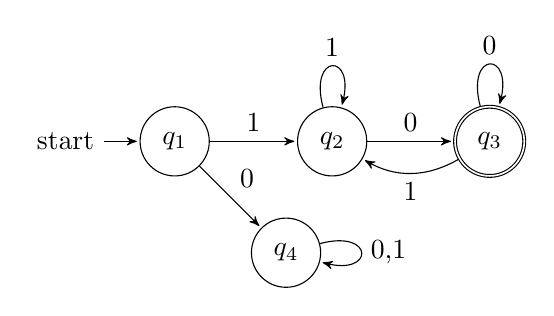
\begin{tikzpicture}[>=stealth', shorten >=1pt, auto, node distance=2cm]

    %define state machine
    \node[initial, state]  (q1) {$q_1$};
    \node[state] (q2) [right of=q1] {$q_2$};
    \node[state, accepting] (q3) [right of=q2] {$q_3$};
    \node[state] (q4) [below right of=q1]{$q_4$};

    %define the links
    \path[->] (q1) edge node{0} (q4)
                   edge node{1} (q2)
              (q2) edge node{0} (q3)
                   edge [loop above] node{1} (q3)
              (q3) edge[loop  above] node{0}(q3)
                  edge [bend left] node{1}(q2)
              (q4) edge [loop right] node{0,1} (q4);
                
  \end{tikzpicture}
\end{center}

\end{document}
